\chapter{Komunikasi Antarlayanan dan Event-Driven Architecture}
\label{ch:ch09}

\section*{Tujuan Pembelajaran}
\begin{itemize}
  \item Membedakan komunikasi sinkron dan asinkron beserta dampaknya terhadap ketersediaan layanan.
  \item Memodelkan proses bisnis sebagai rangkaian \textit{event}.
  \item Membandingkan koordinasi berbasis \textit{choreography} dan \textit{orchestration}.
\end{itemize}

\section{Pendahuluan}

Pada satu Selasa pagi di bulan Maret 2026, layanan pengiriman pesan WhatsApp milik vendor notifikasi
Medikara+ terganggu selama tiga jam. Gangguan itu seharusnya hanya menunda pengingat jadwal.
Kenyataannya, pasien yang menekan tombol "Buat Janji" di Medikara+ melihat pesan gagal. Pada jam
sibuk pukul 07.00 sampai 10.00, Medikara+ biasanya menerima sekitar 175 janji temu per jam, sehingga
sekitar 520 janji temu gagal dibuat pagi itu. Pusat panggilan kewalahan, dan sebagian pasien
memilih berobat ke rumah sakit lain.

Penyebabnya bukan kerusakan di Medikara+ sendiri. Medikara+ memanggil empat sistem secara berurutan
dan menunggu jawaban masing-masing, termasuk layanan notifikasi. Bila satu sistem diam, seluruh alur
ikut berhenti. Pola yang sama berulang pada integrasi \textit{point-to-point} di Medikara Health:
Sistem Informasi Manajemen Rumah Sakit (SIMRS), Enterprise Resource Planning (ERP) keuangan,
jembatan ke BPJS Kesehatan, dan jembatan ke SATUSEHAT saling memanggil secara langsung, sehingga
gangguan di satu titik merambat ke banyak sistem. Bab ini membahas cara layanan berkomunikasi agar
gangguan tidak merambat: kapan sebuah layanan perlu menunggu jawaban, kapan cukup mengirim kabar,
dan bagaimana proses yang melibatkan banyak layanan dikoordinasikan.

\IfFileExists{../figures/ch09-diagram-konsep.png}{%
Broker menyalurkan fakta bisnis kepada konsumen yang berlangganan.
Penyampaian ulang memerlukan identitas event dan pengolahan yang idempoten.
Gambar \ref{fig:ch09-pos-pemilah} merangkum hubungan komponen dan konsep utama bab ini.
\begin{figure}[!htb]
  \centering
  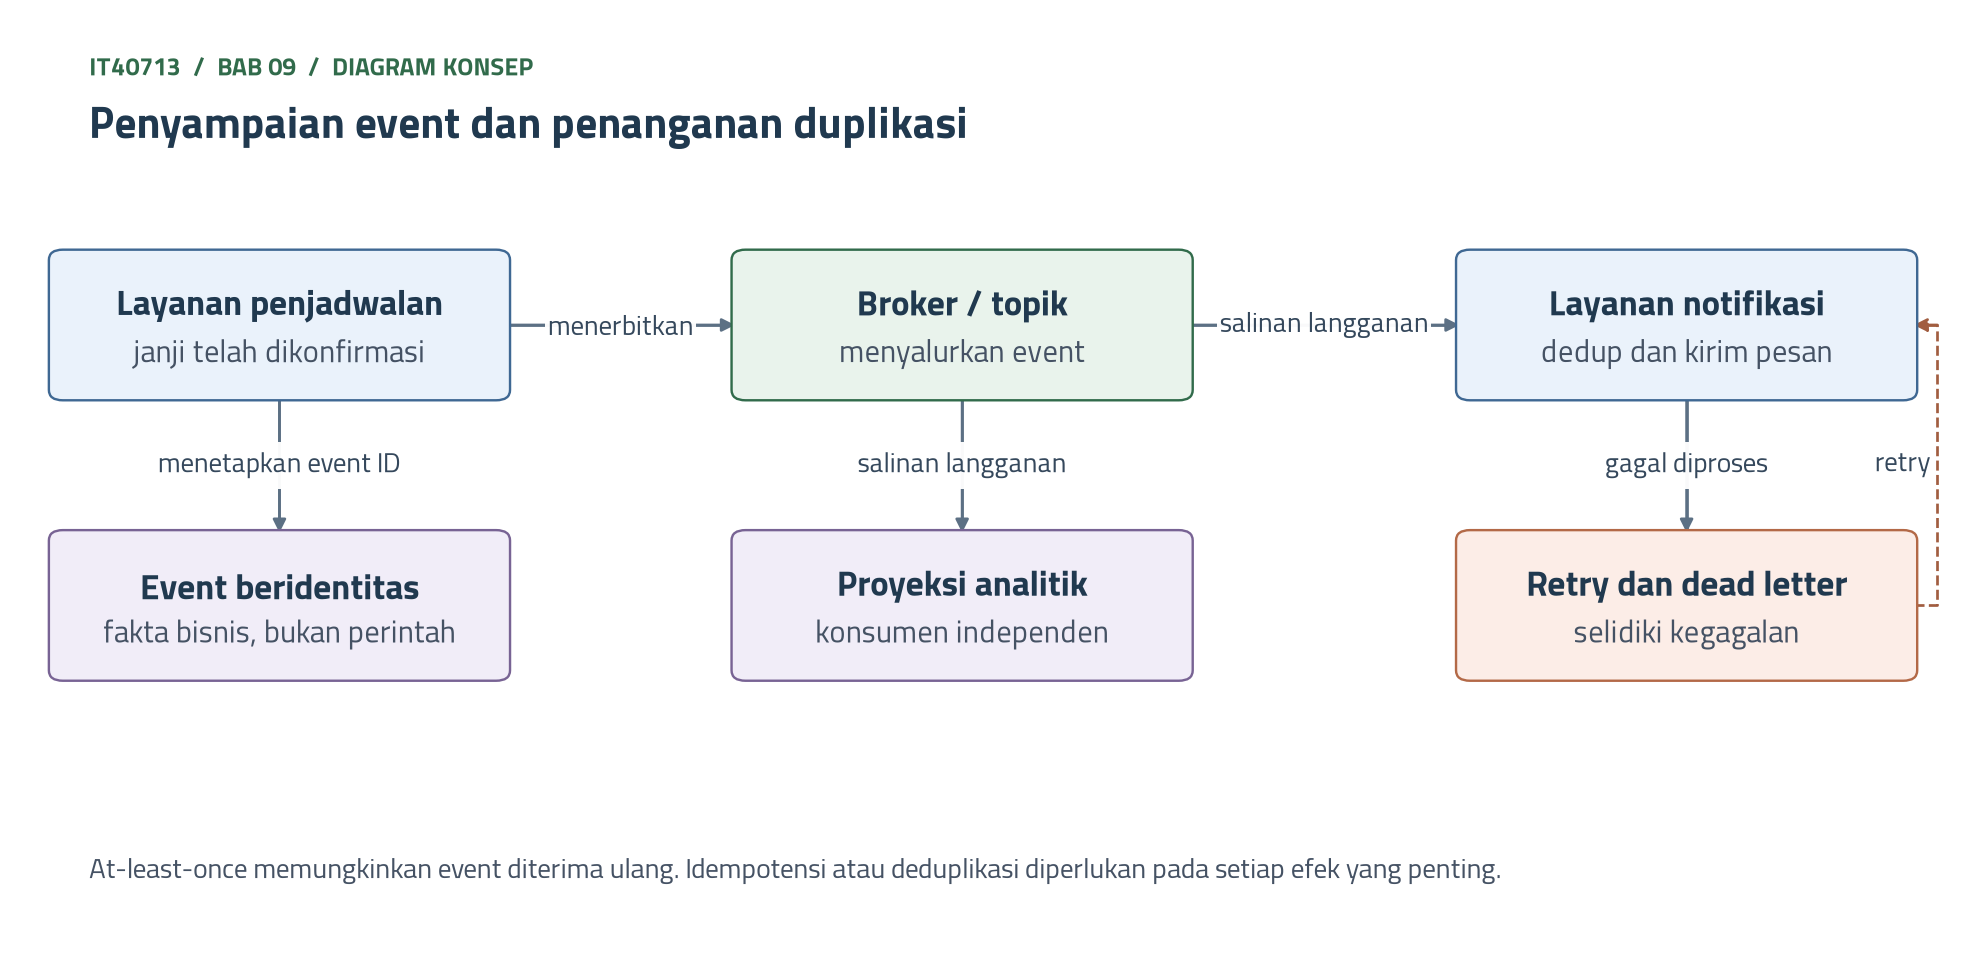
\includegraphics[width=\textwidth]{../figures/ch09-diagram-konsep.png}
  \caption{Penyampaian event dan penanganan duplikasi}
  \label{fig:ch09-pos-pemilah}
\end{figure}%
}{}

Rujukan utama bab ini adalah buku \textit{Building Microservices} karya Newman \cite{newman2021},
\textit{Microservices Patterns} karya Richardson \cite{richardson2018}, katalog pola integrasi
berbasis pesan dari Hohpe dan Woolf \cite{c09-hohpe2003}, serta tulisan Fowler tentang arti
\textit{event-driven} \cite{c09-fowler2017}. Dua spesifikasi terbuka dipakai untuk menuliskan
\textit{event} secara seragam, yaitu CloudEvents \cite{c09-cloudevents} dan AsyncAPI
\cite{c09-asyncapi}. Hasil bab ini adalah peta interaksi layanan dan katalog \textit{event} untuk
tonggak capstone C3.

\section{Komunikasi Sinkron dan Asinkron}
\label{sec:ch09-sinkron}

Komunikasi sinkron terjadi ketika layanan pemanggil mengirim permintaan, lalu berhenti menunggu
jawaban sebelum melanjutkan pekerjaannya. Pola ini disebut \textit{request/response} dan umumnya
berjalan di atas HyperText Transfer Protocol (HTTP), misalnya lewat Application Programming
Interface (API). Syaratnya, pemanggil dan yang dipanggil harus hidup pada saat yang sama. Komunikasi
asinkron terjadi ketika pengirim menitipkan pesan kepada perantara, lalu langsung melanjutkan
pekerjaannya tanpa menunggu. Penerima memproses pesan itu ketika siap. Pengirim dan penerima tidak
harus hidup bersamaan, karena perantara menyimpan pesan sampai diambil \cite{newman2021}.

Analoginya seperti menelepon dan meninggalkan memo. Staf administrasi yang menelepon gudang untuk
menanyakan stok harus menunggu di gagang telepon. Bila gudang tidak mengangkat, pekerjaannya
berhenti. Staf yang meninggalkan memo di kotak masuk gudang bisa langsung kembali bekerja, dan gudang
membaca memo itu setelah rapatnya selesai. Namun memo tidak cocok untuk pertanyaan yang jawabannya
dibutuhkan detik itu juga, misalnya ketika pelanggan sedang menunggu di depan meja.

Tabel \ref{tab:ch09-sinkron-asinkron} merangkum perbedaan keduanya dari sisi yang penting bagi
pemilik layanan.

\begin{table}[!htb]
  \centering
  \caption{Perbandingan komunikasi sinkron dan asinkron}
  \label{tab:ch09-sinkron-asinkron}
  \footnotesize
  \begin{tabularx}{\textwidth}{>{\raggedright\arraybackslash}p{2.4cm} >{\raggedright\arraybackslash}X >{\raggedright\arraybackslash}X}
    \hline
    \textbf{Aspek} & \textbf{Sinkron (\textit{request/response})} & \textbf{Asinkron (lewat
      pesan)} \\ \hline
    Cara kerja & Pemanggil menunggu jawaban & Pengirim menitipkan pesan lalu melanjutkan pekerjaan
      \\ \hline
    Syarat ketersediaan & Semua pihak dalam rantai harus hidup bersamaan & Cukup pengirim dan
      perantara yang hidup; penerima boleh menyusul \\ \hline
    Waktu tunggu pengguna & Jumlah waktu semua panggilan dalam rantai & Hanya waktu menitipkan
      pesan \\ \hline
    Jawaban & Langsung tersedia, termasuk penolakan & Tidak langsung; hasil dikabarkan kemudian
      \\ \hline
    Wujud kegagalan & Pengguna melihat pesan gagal & Pesan menumpuk dan hasil terlambat \\ \hline
    Cocok untuk & Pertanyaan yang jawabannya dibutuhkan saat itu juga & Pekerjaan lanjutan yang
      boleh terlambat beberapa detik atau menit \\ \hline
  \end{tabularx}
\end{table}

Pertanyaan kemudian muncul: seberapa besar pengaruh rantai panggilan sinkron terhadap ketersediaan?
Ketika layanan A memanggil B, lalu B memanggil C, alur itu baru berhasil bila ketiganya hidup.
Ketersediaan gabungannya dihitung sebagai hasil kali ketersediaan setiap mata rantai, dengan anggapan
gangguan masing-masing tidak saling terkait. Waktu tunggunya pun dijumlahkan. Rantai yang panjang
selalu lebih rapuh dan lebih lambat daripada mata rantai terlemahnya.

Keputusan memakai rantai sinkron punya dua konsekuensi. Pertama, ketersediaan alur turun setiap kali
satu sistem ditambahkan ke rantai, walaupun sistem baru itu cukup andal. Empat sistem dengan
ketersediaan 99,5 persen menghasilkan alur dengan ketersediaan sekitar 98 persen, atau sekitar 14 jam
gagal per bulan. Kedua, pemilik alur ikut menanggung gangguan sistem yang tidak dimilikinya. Tim
Medikara+ tidak dapat memperbaiki layanan notifikasi vendor, tetapi keluhan pasien tetap jatuh ke
Medikara+.

Dua contoh dari Medikara Health:
\begin{enumerate}
  \item Pengecekan slot jadwal dokter harus sinkron. Pasien sedang menatap layar dan perlu tahu saat
        itu juga apakah slot Senin pukul 09.30 di poliklinik penyakit dalam masih kosong. Jawaban
        "nanti dikabari" membuat dua pasien bisa memilih slot yang sama.
  \item Pengingat jadwal kontrol sehari sebelum kunjungan cukup asinkron. Sekitar 1.400 pengingat
        terkirim setiap hari kerja, dan pengingat yang terlambat sepuluh menit tidak merugikan
        siapa pun. Pasien tidak perlu menunggu pengingat terkirim untuk menyelesaikan janji
        temunya.
\end{enumerate}

\begin{kasus}[title={Kasus Medikara Health: Alur Janji Temu yang Memanggil Empat Sistem}]
  Saat ini Medikara+ memproses satu janji temu dengan memanggil empat sistem secara berurutan,
  seperti diperlihatkan bagian atas Gambar \ref{fig:ch09-rantai-sinkron}. Pertama, modul jadwal
  dokter di SIMRS mengunci slot. Kedua, jembatan BPJS Kesehatan memeriksa kepesertaan pasien.
  Ketiga, modul pendaftaran SIMRS membuat data kunjungan. Keempat, layanan notifikasi vendor
  mengirim konfirmasi lewat WhatsApp. Ketersediaan bulanan keempatnya menurut catatan tim
  operasi adalah 99,9; 99,0; 99,5; dan 99,0 persen.

  Hasil kalinya sekitar 97,4 persen. Dalam sebulan berisi 43.200 menit, alur janji temu gagal
  sekitar 1.114 menit atau 18,6 jam. Waktu tunggunya juga dijumlahkan: 150 milidetik untuk jadwal,
  1.200 milidetik untuk kepesertaan, 400 milidetik untuk pendaftaran, dan 650 milidetik untuk
  notifikasi, sehingga pasien menunggu sekitar 2,4 detik setiap kali menekan tombol.

  Misalkan alur itu dirancang ulang seperti bagian bawah gambar. Medikara+ hanya menunggu jadwal
  dokter, lalu menitipkan \textit{event} \texttt{JanjiTemuDibuat} ke \textit{event broker}
  terkelola dengan ketersediaan 99,95 persen. Kepesertaan, pendaftaran, dan notifikasi bereaksi
  terhadap \textit{event} itu pada waktunya masing-masing. Ketersediaan yang dirasakan pasien naik
  menjadi sekitar 99,85 persen atau sekitar 65 menit gagal per bulan, dan waktu tunggunya turun
  menjadi sekitar 170 milidetik.

  Rancangan ulang ini punya harga yang harus diputuskan bagian pelayanan, bukan hanya tim TI.
  Pasien BPJS Kesehatan kini mendapat janji temu sebelum kepesertaannya terbukti aktif. Bila
  pemeriksaan kepesertaan gagal, janji temu berubah status menjadi "perlu konfirmasi penjamin" dan
  pasien diberi tahu lewat notifikasi. Keputusan ini sah secara teknis, tetapi hanya pantas
  dijalankan bila bagian pelayanan setuju dan alur penanganan status itu sudah disiapkan.
\end{kasus}

\begin{figure}[!htb]
  \centering
  \begin{tikzpicture}[
  font=\scriptsize,
  panah/.style={-{Stealth[length=2mm]}, thick},
  tahap/.style={draw, rounded corners, fill=blue!8, text width=1.75cm,
    minimum height=0.95cm, align=center},
  tekan/.style={tahap, fill=orange!12},
  induk/.style={draw, rounded corners, fill=praditagreen!15, text width=1.75cm,
    minimum height=0.95cm, align=center},
  pelanggan/.style={draw, rounded corners, fill=blue!8, text width=1.75cm,
    minimum height=0.7cm, align=center},
  judul/.style={font=\footnotesize\bfseries, anchor=west},
  ket/.style={font=\tiny, fill=white, inner sep=1pt}
]
  % Baris A: Medikara+ menunggu empat sistem secara berurutan.
  \node[judul] at (-1.0,0.95) {A. Semua panggilan sinkron};
  \node[tahap] (app1) at (0,0) {Medikara+};
  \node[tahap] (jd1) at (2.4,0) {Jadwal dokter\\{\tiny\mdseries 99,9\%}};
  \node[tahap] (bp1) at (4.8,0) {Kepesertaan BPJS\\{\tiny\mdseries 99,0\%}};
  \node[tahap] (df1) at (7.2,0) {Pendaftaran SIMRS\\{\tiny\mdseries 99,5\%}};
  \node[tekan] (nt1) at (9.6,0) {Notifikasi\\{\tiny\mdseries 99,0\%}};
  \draw[panah] (app1) -- (jd1);
  \draw[panah] (jd1) -- (bp1);
  \draw[panah] (bp1) -- (df1);
  \draw[panah] (df1) -- (nt1);
  \node[draw, rounded corners, fill=red!22, text width=11.0cm, align=center,
    minimum height=0.75cm] at (4.8,-1.2)
    {Ketersediaan gabungan $\approx$ 97,4\%, atau sekitar 18,6 jam gagal per bulan.\\
     Notifikasi yang mati ikut menggagalkan janji temu.};

  % Baris B: hanya jadwal dokter yang ditunggu, sisanya menerima event.
  \node[judul] at (-1.0,-2.15) {B. Hanya jadwal yang sinkron};
  \node[tahap] (app2) at (0,-3.25) {Medikara+};
  \node[tahap] (jd2) at (0,-4.85) {Jadwal dokter\\{\tiny\mdseries 99,9\%}};
  \node[induk] (br) at (3.2,-3.25) {\textit{Event broker}\\{\tiny\mdseries 99,95\%}};
  \node[pelanggan] (bp2) at (6.2,-2.35) {Kepesertaan BPJS};
  \node[pelanggan] (df2) at (6.2,-3.25) {Pendaftaran SIMRS};
  \node[pelanggan, fill=orange!12] (nt2) at (6.2,-4.15)
    {Notifikasi\\{\tiny\mdseries boleh terlambat}};
  \draw[panah] (app2) -- node[ket, right] {sinkron} (jd2);
  \draw[panah] (app2) -- node[ket, above] {\textit{JanjiTemu-}} node[ket, below]
    {\textit{Dibuat}} (br);
  \draw[panah, dashed] (br.east) -- (bp2.west);
  \draw[panah, dashed] (br.east) -- (df2.west);
  \draw[panah, dashed] (br.east) -- (nt2.west);
  \node[draw, rounded corners, fill=green!10, text width=2.6cm, align=center,
    minimum height=0.95cm] at (9.55,-3.25)
    {Yang ditunggu pasien hanya jadwal dan \textit{broker}: $\approx$ 99,85\%,
     sekitar 65 menit per bulan};

  % Keterangan garis.
  \draw[panah] (2.3,-5.35) -- ++(0.6,0);
  \node[anchor=west, font=\tiny] at (3.0,-5.35) {menunggu jawaban};
  \draw[panah, dashed] (5.0,-5.35) -- ++(0.6,0);
  \node[anchor=west, font=\tiny] at (5.7,-5.35) {pesan diantar kemudian};
\end{tikzpicture}

  \caption{Alur janji temu Medikara+: rantai empat panggilan sinkron (A) dibandingkan dengan
           rancangan yang hanya menunggu jadwal dokter dan menitipkan sisanya sebagai
           \textit{event} (B)}
  \label{fig:ch09-rantai-sinkron}
\end{figure}

\section{Antrean Pesan, Publish/Subscribe, dan Event Broker}
\label{sec:ch09-broker}

Komunikasi asinkron membutuhkan perantara. Ada dua bentuk dasar perantara. Antrean pesan
(\textit{point-to-point}) menampung pesan secara berurutan, dan setiap pesan diambil oleh tepat satu
penerima. Bila ada beberapa penerima yang membaca antrean yang sama, mereka berbagi beban: penerima
yang sedang luang mengambil pesan berikutnya. \textit{Publish/subscribe} bekerja dengan topik.
Penerbit mengirim pesan ke satu topik, lalu setiap pelanggan topik itu menerima salinannya sendiri.
Penerbit tidak perlu tahu siapa saja pelanggannya. Hohpe dan Woolf menamai keduanya
\textit{point-to-point channel} dan \textit{publish-subscribe channel} \cite{c09-hohpe2003}.
Perangkat lunak yang menyediakan antrean, topik, atau keduanya disebut \textit{event broker} atau
\textit{message broker}. Tugasnya menerima pesan, menyimpannya dengan aman, dan mengantarkannya
kepada penerima yang berhak.

Analoginya seperti dua cara kantor melayani orang. Antrean pesan mirip nomor antrean di kantor bank:
satu nomor dipanggil oleh satu teller, dan teller yang sedang luang memanggil nomor berikutnya.
\textit{Publish/subscribe} mirip papan pengumuman RT: pengurus menempel satu pengumuman, lalu setiap
warga yang berkepentingan membacanya. Pengurus RT tidak perlu mendatangi rumah warga satu per satu,
dan warga baru cukup ikut membaca papan yang sama. \textit{Event broker} adalah kantor pos yang
mengelola kedua cara itu sekaligus.

Gambar \ref{fig:ch09-antrean-pubsub} memperlihatkan kedua bentuk itu berdampingan.

\begin{figure}[!htb]
  \centering
  \begin{tikzpicture}[
  font=\scriptsize,
  panah/.style={-{Stealth[length=2mm]}, thick},
  tahap/.style={draw, rounded corners, fill=blue!8, text width=1.3cm,
    minimum height=0.8cm, align=center},
  induk/.style={draw, rounded corners, fill=praditagreen!15, text width=1.5cm,
    minimum height=0.95cm, align=center},
  hasil/.style={draw, rounded corners, fill=green!10, text width=1.45cm,
    minimum height=0.7cm, align=center},
  sel/.style={draw, fill=orange!12, minimum width=0.32cm, minimum height=0.5cm},
  judul/.style={font=\footnotesize\bfseries, anchor=west},
  ket/.style={font=\tiny, align=center}
]
  % Panel A: antrean, satu pesan diambil oleh satu penerima.
  \node[judul] at (-0.75,1.55) {A. Antrean pesan};
  \node[tahap] (kirim) at (0,0) {Medikara+\\{\tiny\mdseries pengirim}};
  \foreach \i in {0,1,2,3} {
    \node[sel] (s\i) at (1.45+\i*0.34,0) {};
  }
  \node[draw, dashed, rounded corners, fit=(s0)(s3), inner sep=3pt] (antrean) {};
  \node[ket, above] at (antrean.north) {antrean di \textit{broker}};
  \node[hasil] (p1) at (3.95,0.6) {Pengirim\\pengingat A};
  \node[hasil] (p2) at (3.95,-0.6) {Pengirim\\pengingat B};
  \draw[panah] (kirim) -- (antrean);
  \draw[panah] (antrean.east) -- (p1.west);
  \draw[panah, dashed] (antrean.east) -- (p2.west);
  \node[ket, text width=4.6cm] at (1.75,-1.4)
    {satu pesan diambil satu penerima;\\penerima berbagi beban kerja};

  % Pemisah dua panel.
  \draw[gray!50, dashed] (5.2,1.7) -- (5.2,-1.75);

  % Panel B: publish/subscribe, setiap pelanggan mendapat salinan.
  \node[judul] at (5.45,1.55) {B. \textit{Publish/subscribe}};
  \node[tahap] (terbit) at (6.3,0) {Janji temu\\{\tiny\mdseries penerbit}};
  \node[induk] (topik) at (8.3,0) {Topik\\{\tiny\mdseries \textit{JanjiTemuDibuat}}};
  \node[hasil] (l1) at (10.35,0.95) {Notifikasi};
  \node[hasil] (l2) at (10.35,0) {Pendaftaran};
  \node[hasil] (l3) at (10.35,-0.95) {Analitik};
  \draw[panah] (terbit) -- (topik);
  \draw[panah] (topik.east) -- (l1.west);
  \draw[panah] (topik.east) -- (l2.west);
  \draw[panah] (topik.east) -- (l3.west);
  \node[ket, text width=4.6cm] at (8.3,-1.4)
    {setiap pelanggan mendapat salinan;\\penerbit tidak mengenal pelanggannya};
\end{tikzpicture}

  \caption{Antrean pesan membagi pekerjaan di antara penerima (A), sedangkan
           \textit{publish/subscribe} memberi salinan kepada setiap pelanggan (B)}
  \label{fig:ch09-antrean-pubsub}
\end{figure}

Dua contoh dari Medikara Health:
\begin{enumerate}
  \item Antrean pesan untuk pengiriman pengingat. Sekitar 1.400 pengingat per hari kerja masuk ke
        satu antrean dan dikerjakan oleh dua pengirim. Menjelang kampanye vaksinasi, jumlahnya naik
        menjadi sekitar 4.000 per hari. Tim cukup menambah pengirim ketiga dan keempat tanpa
        mengubah Medikara+ sama sekali.
  \item \textit{Publish/subscribe} untuk \textit{event} janji temu. Notifikasi, pendaftaran SIMRS,
        dan analitik berlangganan topik \texttt{JanjiTemuDibuat}. Selama ini setiap integrasi
        \textit{point-to-point} baru memakan sekitar enam minggu kerja vendor. Dengan topik
        bersama, tim analitik yang membutuhkan data janji temu cukup mendaftar sebagai pelanggan,
        sementara Medikara+ tidak diubah.
\end{enumerate}

Pertanyaan berikutnya: produk apa yang dipakai sebagai \textit{broker}? Pada tingkat konsep, pilihan
umumnya terbagi seperti Tabel \ref{tab:ch09-produk-broker}. Pilihan produk mengikuti keputusan
\textit{runtime} pada Bab 8. \textit{Broker} terkelola mengurangi beban operasi, sedangkan
\textit{broker} yang dijalankan sendiri memberi kendali lebih besar dengan biaya tenaga kerja yang
lebih tinggi. Satu hal tidak boleh terlupa: \textit{broker} ikut menyimpan isi pesan, sehingga aturan
lokasi data dari Bab 2 berlaku juga untuknya.

\begin{table}[!htb]
  \centering
  \caption{Gambaran konsep beberapa produk \textit{broker}}
  \label{tab:ch09-produk-broker}
  \footnotesize
  \begin{tabularx}{\textwidth}{>{\raggedright\arraybackslash}p{2.6cm} >{\raggedright\arraybackslash}X >{\raggedright\arraybackslash}X}
    \hline
    \textbf{Produk} & \textbf{Sifat utama} & \textbf{Cocok untuk} \\ \hline
    RabbitMQ & \textit{Broker} antrean dan topik; pesan dihapus setelah penerima memberi pengakuan &
      Pembagian kerja dan pengantaran pesan dengan aturan rute yang luwes \\ \hline
    Apache Kafka & Log \textit{event} yang disimpan sesuai masa retensi; pelanggan dapat membaca ulang
      dari titik mana pun & Aliran \textit{event} bervolume besar, analitik, dan pelanggan baru yang
      perlu membaca riwayat \\ \hline
    Antrean terkelola (Amazon SQS, Azure Service Bus) & Penyedia \textit{cloud} mengurus server,
      kapasitas, dan pembaruan & Tim kecil yang ingin antrean andal tanpa mengoperasikan
      \textit{broker} \\ \hline
    \textit{Publish/subscribe} terkelola (Google Cloud Pub/Sub, Amazon SNS, Azure Event Grid) &
      Topik terkelola dengan banyak pelanggan & Penyebaran \textit{event} antarlayanan dalam satu
      penyedia \textit{cloud} \\ \hline
  \end{tabularx}
\end{table}

\begin{pendalaman}[title={Pendalaman Teknis (opsional): Menjalankan Broker Lokal}]
  Folder \berkas{sources/chapter09/contoh-broker-lokal} berisi \berkas{docker-compose.yml} untuk
  menjalankan RabbitMQ di komputer sendiri dan skrip \berkas{kirim_terima_event.py} untuk mengirim
  serta menerima \textit{event} \texttt{JanjiTemuDibuat}. RabbitMQ memakai Advanced Message Queuing
  Protocol (AMQP) pada port 5672. Langkahnya:
  \begin{enumerate}
    \item Pasang Docker dan Python 3, lalu masuk ke folder
          \berkas{sources/chapter09/contoh-broker-lokal}.
    \item Jalankan \texttt{docker compose up -d}, kemudian \texttt{pip install pika}.
    \item Jalankan \texttt{python kirim\_terima\_event.py kirim}. Skrip menerbitkan \textit{event}
          yang sama dua kali ke \textit{exchange} \texttt{medikara.janji-temu}.
    \item Buka konsol pengelolaan di \url{http://localhost:15672} dengan pengguna dan sandi
          \texttt{guest}. Antrean \texttt{notifikasi.janji-temu-dibuat} berisi dua pesan.
    \item Jalankan \texttt{python kirim\_terima\_event.py terima}. Pesan pertama diproses, pesan
          kedua dilewati. Alasannya dibahas di Seksi \ref{sec:ch09-idempoten}.
  \end{enumerate}
  \textit{Broker} ini hanya untuk komputer sendiri. Port 5672 dan 15672 tidak boleh dibuka ke
  jaringan publik, dan skrip tidak boleh diarahkan ke \textit{broker} milik organisasi lain tanpa
  izin tertulis.
\end{pendalaman}

\section{Pola Event: Notification, State Transfer, dan Event Sourcing}
\label{sec:ch09-pola-event}

\textit{Event} adalah catatan bahwa sesuatu telah terjadi dalam bisnis, misalnya janji temu dibuat
atau hasil laboratorium selesai divalidasi. Karena sudah terjadi, \textit{event} ditulis dalam
bentuk lampau dan tidak dapat dibatalkan. Kejadian berikutnya hanya dapat mengoreksinya, misalnya
\texttt{JanjiTemuDibatalkan}. Setiap \textit{event} punya satu pemilik, yaitu layanan yang
menerbitkannya.

Dua hal pada pesan sering tertukar: \textit{event} dan perintah. Pembagiannya begini.
\textit{Event} seperti \texttt{JanjiTemuDibuat} menyatakan fakta, dan penerbitnya tidak peduli siapa
yang bereaksi. Perintah seperti \texttt{KirimPengingat} adalah permintaan kepada satu penerima
tertentu, dan penerima itu boleh menolak. Fowler mengingatkan bahaya \textit{event} yang menjadi
perintah terselubung: penerbit diam-diam berharap penerima tertentu melakukan sesuatu, sehingga
keterkaitan yang ingin dihindari muncul kembali \cite{c09-fowler2017}.

Fowler membedakan tiga pola pemakaian \textit{event} \cite{c09-fowler2017}. Pada \textit{event
notification}, \textit{event} hanya membawa kabar singkat dan nomor rujukan. Penerima yang
membutuhkan rincian memanggil balik penerbit. Pada \textit{event-carried state transfer},
\textit{event} membawa data yang berubah, sehingga penerima dapat menyimpan salinannya dan tidak perlu
memanggil balik. Pada \textit{event sourcing}, setiap perubahan status disimpan sebagai rangkaian
\textit{event}, dan status saat ini dihitung dengan memutar ulang seluruh rangkaian itu.

Analoginya seperti tiga cara bank memberi kabar. Pesan singkat "ada transaksi di rekening, silakan
cek aplikasi" adalah \textit{event notification}: nasabah harus membuka aplikasi untuk tahu
rinciannya. Pesan yang langsung memuat nominal, tujuan, dan saldo akhir adalah \textit{event-carried
state transfer}: nasabah tidak perlu membuka aplikasi. Buku tabungan adalah \textit{event sourcing}:
saldo tidak ditulis sebagai satu angka, melainkan dihitung dari seluruh baris mutasi sejak rekening
dibuka.

Tabel \ref{tab:ch09-pola-event} merangkum kelebihan dan biaya setiap pola.

\begin{table}[!htb]
  \centering
  \caption{Tiga pola pemakaian \textit{event} menurut Fowler \cite{c09-fowler2017}}
  \label{tab:ch09-pola-event}
  \footnotesize
  \begin{tabularx}{\textwidth}{>{\raggedright\arraybackslash}p{2.1cm} >{\raggedright\arraybackslash}X >{\raggedright\arraybackslash}X >{\raggedright\arraybackslash}X}
    \hline
    \textbf{Pola} & \textbf{Isi \textit{event}} & \textbf{Kelebihan} & \textbf{Biaya} \\ \hline
    \textit{Event notification} & Kabar singkat dan nomor rujukan & Keterkaitan rendah; data
      sensitif tetap di pemiliknya & Alur logis tidak terlihat di satu tempat; panggilan balik
      menambah beban penerbit \\ \hline
    \textit{Event-carried state transfer} & Data yang berubah, cukup untuk dipakai penerima & Penerima
      tetap bekerja walaupun penerbit mati; waktu tunggu pendek & Data tersalin di banyak tempat;
      salinan bisa sementara tertinggal; data pribadi ikut menyebar \\ \hline
    \textit{Event sourcing} & Seluruh perubahan status sebagai rangkaian \textit{event} & Jejak audit
      lengkap; kondisi masa lalu dapat direkonstruksi & Rumit; perubahan bentuk \textit{event} dan
      pemutaran ulang yang melibatkan sistem luar sulit ditangani \\ \hline
  \end{tabularx}
\end{table}

Keputusan memilih pola punya dua konsekuensi. Pertama, \textit{event-carried state transfer}
membuat data tersebar, sehingga pertanyaan "siapa saja yang menyimpan data pasien ini" makin sulit
dijawab. Pertanyaan itu wajib terjawab menurut Undang-Undang Pelindungan Data Pribadi (UU PDP)
\cite{uu27-2022-pdp}. Kedua, \textit{event sourcing} adalah keputusan penyimpanan data, bukan
sekadar keputusan komunikasi. Pola ini layak dipertimbangkan bila jejak audit lengkap memang
dibutuhkan, misalnya pada riwayat perubahan rekam medis, dan tidak perlu dipakai di semua layanan.

Nama \textit{event} sebaiknya memakai bahasa bisnis yang sama dengan \textit{ubiquitous language}
pada Bab 6 \cite{evans2003}. Nama yang baik ditulis dalam bentuk lampau dan dipahami bagian
pelayanan, misalnya \texttt{HasilLabTersedia}. Nama teknis seperti \texttt{RecordUpdated} atau
\texttt{StatusChanged} memaksa setiap pelanggan menebak artinya. Papan EventStorming yang disusun
tim pada Bab 6 adalah sumber terbaik nama \textit{event}, karena kejadian berwarna oranye di papan
itu sudah ditulis dalam bahasa bisnis.

Dua contoh dari Medikara Health:
\begin{enumerate}
  \item Laboratorium rujukan memvalidasi sekitar 2.600 hasil pemeriksaan per hari. Hasil
        laboratorium adalah data kesehatan yang sensitif, sehingga \texttt{HasilLabTersedia}
        cukup membawa nomor permintaan dan penanda kritis. Dokter yang berhak mengambil isinya lewat
        API yang memeriksa hak akses.
  \item Penagihan menerbitkan sekitar 3.300 tagihan per hari. ERP keuangan membutuhkan nomor
        tagihan, total, dan penjamin, tetapi tidak membutuhkan data klinis. \texttt{TagihanTerbit}
        membawa data itu secara lengkap, sehingga ERP tidak perlu memanggil balik Penagihan.
\end{enumerate}

\begin{kasus}[title={Kasus Medikara Health: Tiga Event Pertama}]
  Tim transformasi menetapkan tiga \textit{event} pertama untuk alur janji temu sampai tagihan.
  Ketiganya diambil dari papan EventStorming Bab 6 dan dirangkum pada Tabel
  \ref{tab:ch09-event-medikara}. Polanya sengaja berbeda-beda, karena kebutuhan pelanggannya juga
  berbeda.

  \texttt{JanjiTemuDibuat} memakai \textit{event notification} yang membawa sebagian data. Data itu
  cukup bagi notifikasi untuk menjadwalkan pengingat, tetapi identitas pasien hanya berupa nomor
  rujukan. \texttt{HasilLabTersedia} sengaja memakai \textit{event notification} murni. Keputusan
  ini menjawab temuan audit internal tentang kontrol akses yang lemah: isi hasil laboratorium tidak
  ikut tersebar ke semua pelanggan. \texttt{TagihanTerbit} memakai \textit{event-carried state
  transfer}, karena isinya data keuangan tanpa data klinis dan pelanggannya perlu tetap bekerja
  saat Penagihan sedang dipelihara.
\end{kasus}

\begin{table}[!htb]
  \centering
  \caption{Tiga \textit{event} pertama Medikara Health (angka rekaan)}
  \label{tab:ch09-event-medikara}
  \footnotesize
  \begin{tabularx}{\textwidth}{>{\raggedright\arraybackslash}p{2.3cm} >{\raggedright\arraybackslash}p{1.8cm} >{\raggedright\arraybackslash}X >{\raggedright\arraybackslash}X r}
    \hline
    \textbf{\textit{Event}} & \textbf{Pemilik} & \textbf{Isi data} & \textbf{Pelanggan} &
      \textbf{Per hari} \\ \hline
    \texttt{JanjiTemu\-Dibuat} & Janji temu (Medikara+) & Nomor janji temu, rujukan pasien,
      fasilitas, poliklinik, waktu & Notifikasi, pendaftaran, kepesertaan, analitik & 1.400 \\
      \hline
    \texttt{HasilLab\-Tersedia} & Laboratorium & Nomor permintaan, rujukan pasien, penanda kritis &
      Pelayanan klinis, notifikasi, penagihan & 2.600 \\ \hline
    \texttt{Tagihan\-Terbit} & Penagihan & Nomor tagihan, nomor kunjungan, total, penjamin &
      Notifikasi, ERP keuangan, klaim & 3.300 \\ \hline
  \end{tabularx}
\end{table}

\begin{pendalaman}[title={Pendalaman Teknis (opsional): CloudEvents dan AsyncAPI}]
  CloudEvents adalah spesifikasi netral vendor untuk format data \textit{event}. Versi rilis
  terakhirnya 1.0.2, dan proyeknya berstatus \textit{graduated} di Cloud Native Computing
  Foundation (CNCF) sejak Januari 2024 \cite{c09-cloudevents}. Spesifikasi ini mewajibkan empat
  atribut: \texttt{id}, \texttt{source}, \texttt{specversion}, dan \texttt{type}. Atribut
  \texttt{time}, \texttt{subject}, \texttt{datacontenttype}, dan \texttt{dataschema} bersifat
  pilihan. Pasangan \texttt{source} dan \texttt{id} yang sama menandai \textit{event} yang sama,
  sehingga penerima dapat mengenali kiriman ganda.

  AsyncAPI 3.0.0 menggambarkan API berbasis pesan dalam format yang dapat dibaca mesin dan tidak
  terikat pada protokol tertentu \cite{c09-asyncapi}. Dokumennya memuat \textit{channel} sebagai
  alamat pesan, \textit{operation} dengan aksi \texttt{send} atau \texttt{receive}, dan
  \textit{message} beserta isinya. Listing \ref{lst:ch09-asyncapi} memperlihatkan definisi pesan
  \texttt{JanjiTemuDibuat} yang memakai amplop CloudEvents. Berkas lengkapnya ditulis dalam YAML
  Ain't Markup Language (YAML) dan dapat dijadikan pola katalog \textit{event} dalam format mesin.

\begin{lstlisting}[language=yaml, captionpos=b, xleftmargin=1.6em,
  caption={Definisi pesan \texttt{JanjiTemuDibuat} dalam AsyncAPI, tersedia di \berkas{sources/chapter09/asyncapi-janji-temu.yaml}},
  label={lst:ch09-asyncapi}]
components:
  messages:
    JanjiTemuDibuat:
      name: JanjiTemuDibuat
      title: Janji temu dibuat
      contentType: application/cloudevents+json
      payload:
        type: object
        required: [specversion, id, source, type, time, data]
        properties:
          specversion:
            type: string
            const: '1.0'
          id:
            type: string
            description: Kunci idempotensi saat dikirim ulang.
          source:
            type: string
            const: /medikara-plus/janji-temu
          type:
            type: string
            const: example.medikara.janjitemu.dibuat.v1
\end{lstlisting}
\end{pendalaman}

\section{Choreography dan Orchestration}
\label{sec:ch09-koordinasi}

Proses bisnis yang melibatkan banyak layanan perlu dikoordinasikan. Ada dua cara.
\textit{Choreography} tidak memakai pengatur pusat. Setiap layanan mendengarkan \textit{event} yang
relevan, memutuskan sendiri reaksinya, lalu menerbitkan \textit{event} baru bila perlu. Alur proses
muncul dari gabungan reaksi itu. \textit{Orchestration} memakai satu komponen pengatur yang disebut
orkestrator. Orkestrator mengetahui urutan langkah, memanggil atau mengirim perintah ke setiap
layanan, menyimpan status proses, dan menangani batas waktu serta kegagalan
\cite{newman2021,richardson2018}.

Analoginya seperti kerja bakti dan renovasi rumah. Kerja bakti di lingkungan RT berjalan tanpa
mandor: warga melihat selokan sudah dibersihkan, lalu mengangkut sampahnya, lalu warga lain mengecat
pagar. Tidak ada yang memerintah, tetapi juga tidak ada yang tahu persis kapan semuanya selesai.
Renovasi rumah memakai mandor yang memegang daftar pekerjaan, memanggil tukang listrik setelah
tembok berdiri, dan menjadi satu-satunya orang yang bisa ditanya "sudah sampai mana".

Gambar \ref{fig:ch09-koreografi-orkestrasi} memperlihatkan kedua cara itu pada kasus Medikara Health.

\begin{figure}[!htb]
  \centering
  \begin{tikzpicture}[
  font=\scriptsize,
  panah/.style={-{Stealth[length=2mm]}, thick},
  tahap/.style={draw, rounded corners, fill=blue!8, text width=1.6cm,
    minimum height=0.8cm, align=center},
  induk/.style={draw, rounded corners, fill=praditagreen!15, text width=1.7cm,
    minimum height=1.0cm, align=center},
  judul/.style={font=\footnotesize\bfseries, anchor=west},
  ket/.style={font=\tiny, fill=white, inner sep=1pt, align=center},
  nomor/.style={circle, draw, fill=orange!12, font=\tiny\bfseries, inner sep=1pt}
]
  % Panel A: choreography, tiap layanan bereaksi pada event di broker.
  \node[judul] at (-0.6,2.35) {A. \textit{Choreography}};
  \node[draw, rounded corners, fill=praditagreen!15, minimum width=5.4cm,
    minimum height=0.5cm] (bus) at (2.2,0) {\textit{event broker}};
  \node[tahap] (jt) at (0.6,1.5) {Janji temu};
  \node[tahap] (lab) at (3.8,1.5) {Laboratorium};
  \node[tahap] (nt) at (0.1,-1.5) {Notifikasi};
  \node[tahap] (df) at (2.2,-1.5) {Pendaftaran};
  \node[tahap] (rm) at (4.3,-1.5) {Pelayanan klinis};
  \draw[panah] (jt) -- node[ket] {\textit{JanjiTemuDibuat}} (jt |- bus.north);
  \draw[panah] (lab) -- node[ket] {\textit{HasilLabTersedia}} (lab |- bus.north);
  \draw[panah, dashed] (nt |- bus.south) -- (nt);
  \draw[panah, dashed] (df |- bus.south) -- (df);
  \draw[panah, dashed] (rm |- bus.south) -- (rm);
  \node[ket, text width=5.2cm] at (2.2,-2.45)
    {tanpa pengatur pusat; alur tersebar di banyak layanan};

  % Pemisah dua panel.
  \draw[gray!50, dashed] (5.45,2.5) -- (5.45,-2.7);

  % Panel B: orchestration, satu pengatur memanggil langkah secara berurutan.
  \node[judul] at (5.7,2.35) {B. \textit{Orchestration}};
  \node[induk] (ork) at (8.45,0) {Orkestrator klaim\\{\tiny\mdseries menyimpan status}};
  \node[tahap] (polis) at (6.65,1.5) {Mitra asuransi\\{\tiny\mdseries cek polis}};
  \node[tahap] (resume) at (10.25,1.5) {Pelayanan klinis\\{\tiny\mdseries resume medis}};
  \node[tahap] (biaya) at (6.65,-1.5) {Penagihan\\{\tiny\mdseries rincian biaya}};
  \node[tahap] (erp) at (10.25,-1.5) {ERP keuangan\\{\tiny\mdseries catat piutang}};
  \draw[panah] (ork) -- node[nomor] {1} (polis);
  \draw[panah] (ork) -- node[nomor] {2} (resume);
  \draw[panah] (ork) -- node[nomor] {3} (biaya);
  \draw[panah] (ork) -- node[nomor] {4} (erp);
  \node[ket, text width=5.2cm] at (8.45,-2.45)
    {satu pengatur menentukan urutan dan status klaim};
\end{tikzpicture}

  \caption{\textit{Choreography} untuk reaksi atas janji temu dan hasil laboratorium (A), serta
           \textit{orchestration} untuk proses klaim asuransi (B)}
  \label{fig:ch09-koreografi-orkestrasi}
\end{figure}

Tabel \ref{tab:ch09-koordinasi} membandingkan keduanya. Perbedaan terbesarnya ada pada
\textit{tradeoff} antara kebebasan setiap layanan dan kemudahan melacak alur.

\begin{table}[!htb]
  \centering
  \caption{Perbandingan \textit{choreography} dan \textit{orchestration}}
  \label{tab:ch09-koordinasi}
  \footnotesize
  \begin{tabularx}{\textwidth}{>{\raggedright\arraybackslash}p{2.4cm} >{\raggedright\arraybackslash}X >{\raggedright\arraybackslash}X}
    \hline
    \textbf{Aspek} & \textbf{\textit{Choreography}} & \textbf{\textit{Orchestration}} \\ \hline
    Keterkaitan & Rendah; layanan hanya mengenal \textit{event} & Orkestrator mengenal semua layanan
      yang dipanggilnya \\ \hline
    Melacak alur & Sulit; alur tersebar di banyak layanan & Mudah; status setiap proses ada di
      orkestrator \\ \hline
    Menambah reaksi baru & Mudah; cukup berlangganan \textit{event} & Orkestrator harus diubah \\
      \hline
    Urutan ketat dan batas waktu & Sulit dijamin & Diatur di satu tempat \\ \hline
    Risiko utama & Alur yang tidak dipahami siapa pun & Orkestrator menjadi pusat logika yang
      gemuk \\ \hline
    Cocok untuk & Reaksi lepas antar-\textit{bounded context} & Proses bisnis berurutan dengan
      status, batas waktu, dan langkah pembatalan \\ \hline
  \end{tabularx}
\end{table}

Pertanyaan kemudian muncul: kapan memilih masing-masing? Tiga pertanyaan membantu. Pertama, apakah
urutan langkah penting dan ada batas waktu yang harus dipantau? Bila ya, \textit{orchestration} lebih
aman. Kedua, apakah ada orang yang harus bisa menjawab "proses ini sudah sampai mana"? Bila ya,
status proses perlu disimpan di satu tempat. Ketiga, apakah reaksi-reaksinya saling lepas dan sering
bertambah? Bila ya, \textit{choreography} lebih luwes. Dalam satu organisasi, kedua cara biasanya
dipakai bersama: \textit{choreography} di antara \textit{bounded context}, dan \textit{orchestration}
di dalam satu proses bisnis yang panjang \cite{newman2021}.

Dua contoh dari Medikara Health:
\begin{enumerate}
  \item Reaksi atas \texttt{JanjiTemuDibuat} memakai \textit{choreography}. Notifikasi, pendaftaran,
        dan analitik bereaksi sendiri-sendiri. Ketika bagian pemasaran ingin mengirim survei
        kepuasan tiga hari setelah kunjungan, layanan survei cukup berlangganan \textit{event} yang
        sudah ada.
  \item Proses klaim asuransi memakai \textit{orchestration}. Prosesnya berurutan, menunggu jawaban
        mitra sampai berhari-hari, dan petugas klaim harus bisa menjawab pertanyaan rumah sakit
        tentang posisi setiap klaim. Rinciannya ada pada kotak kasus berikut.
\end{enumerate}

\begin{kasus}[title={Kasus Medikara Health: Klaim dari Mitra Asuransi sebagai Orchestration}]
  Medikara Health bekerja sama dengan 9 perusahaan asuransi mitra dan mengajukan sekitar 3.600 klaim
  rawat jalan per bulan. Setiap klaim melewati empat langkah, sesuai bagian kanan Gambar
  \ref{fig:ch09-koreografi-orkestrasi}: memeriksa polis dan manfaat lewat API mitra asuransi,
  mengambil resume medis dan kode diagnosis dari Pelayanan klinis, mengambil rincian biaya dari
  Penagihan, lalu mencatat piutang di ERP keuangan setelah keputusan mitra keluar. Keputusan mitra
  rata-rata keluar dalam 11 hari kerja.

  Misalkan proses ini disusun dengan \textit{choreography}. Status satu klaim akan tersebar di lima
  layanan, dan petugas klaim harus menelusuri lima catatan untuk menjawab satu telepon. Klaim yang
  macet di mitra juga tidak akan terdeteksi, karena tidak ada komponen yang menunggu jawaban
  tersebut. Karena itu tim memilih \textit{orchestration}. Layanan Klaim Asuransi menjadi
  orkestrator di \textit{bounded context} Klaim. Layanan ini menyimpan status setiap klaim,
  mengingatkan petugas bila mitra belum menjawab dalam 14 hari kerja, dan menjalankan langkah
  pembatalan bila salah satu langkah gagal. Rancangan langkah pembatalan itu dibahas pada Bab 10.
\end{kasus}

\section{Pengiriman At-Least-Once dan Idempotensi}
\label{sec:ch09-idempoten}

Setiap \textit{broker} memberi jaminan pengiriman tertentu. Jaminan \textit{at-most-once} (paling
banyak sekali) mengirim pesan tanpa menunggu pengakuan dari penerima. Pesan tidak pernah ganda,
tetapi bisa hilang. Jaminan \textit{at-least-once} (paling sedikit sekali) mengirim ulang pesan
sampai penerima memberi pengakuan (\textit{acknowledgement}). Pesan tidak hilang, tetapi bisa
diterima lebih dari sekali. Jaminan \textit{exactly-once} (tepat sekali) menjanjikan pesan diproses
tepat satu kali. Janji ini sulit dipenuhi secara menyeluruh di jaringan yang bisa putus kapan saja,
sehingga produk yang menawarkannya biasanya membatasinya pada lingkup platform itu sendiri.

Pertanyaan kemudian muncul: mengapa pesan bisa terkirim dua kali? Ada dua penyebab yang umum.
Pertama, penerima sudah selesai memproses pesan, tetapi koneksi putus sebelum pengakuannya sampai.
\textit{Broker} menganggap pesan belum diproses, lalu mengirimkannya lagi. Kedua, pengirim tidak
menerima konfirmasi dari \textit{broker}, lalu mengulang pengirimannya. Dokumentasi RabbitMQ
menyatakan bahwa pengakuan menjamin pengiriman \textit{at-least-once}, bahwa penerima harus siap
menerima pesan yang pernah dilihatnya, dan bahwa penerima sebaiknya dirancang idempoten
\cite{c09-rabbitmq-reliability}. Tabel \ref{tab:ch09-jaminan} merangkum ketiga jaminan itu.

\begin{table}[!htb]
  \centering
  \caption{Tiga jaminan pengiriman pesan}
  \label{tab:ch09-jaminan}
  \footnotesize
  \begin{tabularx}{\textwidth}{>{\raggedright\arraybackslash}p{2.2cm} >{\raggedright\arraybackslash}X >{\raggedright\arraybackslash}X >{\raggedright\arraybackslash}X}
    \hline
    \textbf{Jaminan} & \textbf{Arti} & \textbf{Risiko} & \textbf{Contoh pemakaian} \\ \hline
    \textit{At-most-once} & Dikirim sekali tanpa pengakuan & Pesan bisa hilang & Data telemetri yang
      segera tergantikan data berikutnya \\ \hline
    \textit{At-least-once} & Dikirim ulang sampai diakui & Pesan bisa ganda & Sebagian besar
      \textit{event} bisnis, dipasangkan dengan penerima yang idempoten \\ \hline
    \textit{Exactly-once} & Diproses tepat sekali & Berlaku terbatas dalam satu platform; mahal &
      Pengolahan aliran data di dalam satu platform \\ \hline
  \end{tabularx}
\end{table}

Penerima yang idempoten menghasilkan keadaan akhir yang sama, baik pesan diproses sekali maupun
berkali-kali. Ada tiga cara umum untuk mencapainya. Pertama, penerima mencatat \texttt{id} setiap
\textit{event} yang sudah diproses dan melewati \texttt{id} yang sama. Kedua, operasi ditulis
sebagai "tetapkan nilai" dan bukan "tambahkan nilai". Ketiga, basis data menolak data ganda lewat
kunci unik, misalnya nomor tagihan. Hohpe dan Woolf menyebut penerima seperti ini
\textit{idempotent receiver} \cite{c09-hohpe2003}.

Analoginya seperti tombol pemanggil lift. Tombol ditekan sekali atau lima kali, lift tetap datang
satu kali. Sebaliknya, kasir yang mencatat setiap struk yang diserahkan tanpa memeriksa nomornya akan
mencatat pembayaran yang sama dua kali bila pelanggan menyerahkan fotokopi struknya.

Pertanyaan berikutnya: siapa yang bertanggung jawab atas idempotensi? Jawabannya penerima, karena
\textit{broker} tidak tahu arti bisnis sebuah pesan. Pengirim membantu dengan memberi \texttt{id}
yang tetap sama pada setiap pengiriman ulang. Tanpa \texttt{id} yang tetap, penerima tidak bisa
membedakan kiriman ulang dari kejadian baru.

Dua contoh dampak bisnis dari Medikara Health:
\begin{enumerate}
  \item Misalkan layanan pengirim tagihan tidak idempoten, dan 0,1 persen dari sekitar 100.000
        \textit{event} \texttt{TagihanTerbit} per bulan diterima dua kali. Hasilnya sekitar 100
        tagihan ganda per bulan. Dengan rata-rata tagihan Rp385.000, pasien dan perusahaan klien
        menerima tagihan berlebih sekitar Rp38,5 juta per bulan, belum termasuk waktu petugas
        untuk mengoreksi dan menjawab keluhan.
  \item Pengingat jadwal yang terkirim dua kali hanya mengganggu pasien, dan biaya per pesannya
        kecil. Karena itu tim memprioritaskan idempotensi pada penerima yang menyentuh uang dan
        rekam medis, lalu menyusul pada penerima lain.
\end{enumerate}

\begin{pendalaman}[title={Pendalaman Teknis (opsional): Penerima yang Idempoten}]
  Skrip pada Seksi \ref{sec:ch09-broker} mengirim \textit{event} yang sama dua kali. Listing
  \ref{lst:ch09-idempoten} memperlihatkan cara penerimanya melewati kiriman kedua. \texttt{id}
  \textit{event} dicatat ke tabel SQLite berkunci primer. Penyisipan kedua dengan \texttt{id} yang
  sama ditolak basis data, sehingga pemeriksaan dan pencatatan terjadi dalam satu langkah. Pesan
  duplikat tetap diakui agar \textit{broker} tidak terus mengirimnya. Pada sistem nyata, pencatatan
  \texttt{id} dan efek bisnisnya disimpan dalam satu transaksi. Pola yang menjaga keduanya tetap
  sejalan dibahas pada Bab 10.

\begin{lstlisting}[language=Python, basicstyle=\ttfamily\scriptsize,
  keywordstyle=\color{blue}\bfseries, commentstyle=\color{gray}\itshape,
  stringstyle=\color{red}, frame=lines, numbers=left,
  numberstyle=\tiny\color{gray}, backgroundcolor=\color{lightgray!10},
  breaklines=true, showstringspaces=false, captionpos=b, xleftmargin=1.6em,
  caption={Penerima yang melewati \textit{event} ganda, tersedia di \berkas{sources/chapter09/contoh-broker-lokal/kirim_terima_event.py}},
  label={lst:ch09-idempoten}]
def tandai_terproses(catatan, id_event):
  """Mencatat id event; False berarti id itu sudah pernah dicatat.

  Pemeriksaan dan pencatatan terjadi dalam satu perintah INSERT,
  sehingga dua penerima yang berjalan bersamaan tidak sama-sama
  lolos.
  """
  try:
    with catatan:
      catatan.execute(
        "INSERT INTO event_terproses (id) VALUES (?)", (id_event,)
      )
    return True
  except sqlite3.IntegrityError:
    return False


def terima_event():
  """Mengambil semua pesan dan memproses setiap event sekali saja.

  Pesan duplikat tetap diakui (ack) agar broker tidak mengirimnya
  terus. Pada sistem nyata, pencatatan id dan efek bisnisnya
  disimpan dalam satu transaksi; contoh ini menyederhanakannya.
  """
  koneksi, kanal = buka_kanal()
  catatan = buka_catatan_terproses()
  while True:
    metode, _properti, isi = kanal.basic_get(queue=NAMA_ANTREAN)
    if metode is None:
      break
    event = json.loads(isi)
    if tandai_terproses(catatan, event["id"]):
      nomor = event["data"]["nomorJanjiTemu"]
      print(f"Proses: pengingat untuk {nomor} dikirim")
    else:
      print(f"Lewati: event {event['id']} sudah pernah diproses")
    kanal.basic_ack(delivery_tag=metode.delivery_tag)
  catatan.close()
  koneksi.close()
\end{lstlisting}
\end{pendalaman}

\section{Service Mesh dan Batas dengan Desain API}
\label{sec:ch09-mesh}

Ketika jumlah layanan bertambah, setiap layanan perlu mengurus hal yang sama: mengenkripsi
lalu lintas, mengulang panggilan yang gagal (\textit{retry}), membatasi waktu tunggu, dan mencatat
telemetri. \textit{Service mesh} memindahkan urusan itu dari kode aplikasi ke lapisan infrastruktur.
Dokumentasi Istio mendefinisikannya sebagai lapisan infrastruktur yang memberi aplikasi kemampuan
keamanan \textit{zero-trust}, \textit{observability}, dan pengaturan lalu lintas tanpa perubahan
kode \cite{c09-istio-mesh}. Caranya, setiap layanan ditemani \textit{proxy} yang mencegat semua
lalu lintas masuk dan keluar. Pola ini dikenal sebagai \textit{sidecar}. \textit{Control plane}
membagikan aturan dan sertifikat kepada semua \textit{proxy}. Enkripsi dua arah antarlayanan yang
dijalankan \textit{proxy} disebut mutual Transport Layer Security (mTLS).

Analoginya seperti gedung perkantoran yang dikelola bersama. Setiap penyewa tidak perlu menyewa
satpam, memasang kamera, dan mencetak kartu akses sendiri. Pengelola gedung menyediakan satpam di
setiap lantai, kartu akses, dan kamera yang terhubung ke satu ruang pantau. Satpam di lobi depan
yang memeriksa tamu dari luar gedung adalah urusan lain, dan perannya mirip \textit{API gateway}.

Gambar \ref{fig:ch09-service-mesh} memperlihatkan pembagian itu. \textit{API gateway} mengurus lalu
lintas dari luar ke dalam sistem, yang lazim disebut utara-selatan. \textit{Service mesh} mengurus
lalu lintas antarlayanan di dalam sistem, yang disebut timur-barat.

\begin{figure}[!htb]
  \centering
  \begin{tikzpicture}[
  font=\scriptsize,
  panah/.style={-{Stealth[length=2mm]}, thick},
  tahap/.style={draw, rounded corners, fill=blue!8, text width=1.6cm,
    minimum height=0.75cm, align=center},
  tekan/.style={tahap, fill=orange!12},
  induk/.style={draw, rounded corners, fill=praditagreen!15, text width=2.4cm,
    minimum height=0.8cm, align=center},
  proksi/.style={draw, rounded corners, fill=green!10, text width=1.6cm,
    minimum height=0.6cm, align=center},
  ket/.style={font=\tiny, align=center},
  atur/.style={-{Stealth[length=1.6mm]}, dashed, praditagreen!80!black}
]
  % Lalu lintas dari luar masuk lewat API gateway di tepi sistem.
  \node[tahap, fill=white] (mitra) at (0,0.5) {Aplikasi mitra\\{\tiny\mdseries asuransi}};
  \node[tekan] (gw) at (2.45,0.5) {\textit{API gateway}\\{\tiny\mdseries tepi sistem}};

  % Dua layanan, masing-masing ditemani proxy sidecar.
  \node[proksi] (px1) at (5.2,0.5) {\textit{proxy}};
  \node[tahap] (app1) at (5.2,-0.6) {Layanan Klaim};
  \node[proksi] (px2) at (9.0,0.5) {\textit{proxy}};
  \node[tahap] (app2) at (9.0,-0.6) {Layanan Rekam Medis};
  \node[draw, rounded corners, gray!70, fit=(px1)(app1), inner sep=3pt] (pod1) {};
  \node[draw, rounded corners, gray!70, fit=(px2)(app2), inner sep=3pt] (pod2) {};
  \draw[{Stealth[length=1.6mm]}-{Stealth[length=1.6mm]}] (px1) -- (app1);
  \draw[{Stealth[length=1.6mm]}-{Stealth[length=1.6mm]}] (px2) -- (app2);

  % Control plane membagikan aturan ke semua proxy.
  \node[induk] (cp) at (7.1,2.0) {\textit{Control plane}\\{\tiny\mdseries aturan dan sertifikat}};
  \draw[atur] (cp.west) -| (px1.north);
  \draw[atur] (cp.east) -| (px2.north);

  % Lalu lintas utara-selatan dan timur-barat.
  \draw[panah] (mitra) -- (gw);
  \draw[panah] (gw) -- (px1);
  \draw[panah] (px1) -- (px2);
  \node[ket, above] at (1.25,1.12) {utara-selatan};
  \node[ket, above] at (7.1,0.55) {timur-barat};
  \node[ket] at (7.1,0.05) {mTLS, \textit{retry},\\telemetri};

  % Batas klaster yang memakai service mesh.
  \node[draw, dashed, thick, praditagreen, rounded corners, inner sep=6pt,
    fit=(pod1)(pod2)(cp)] (klaster) {};
  \node[font=\tiny\bfseries, praditagreen, anchor=north west] at (klaster.south west)
    {klaster dengan \textit{service mesh}};
\end{tikzpicture}

  \caption{\textit{API gateway} di tepi sistem dan \textit{service mesh} untuk lalu lintas
           antarlayanan, dengan \textit{proxy} di samping setiap layanan}
  \label{fig:ch09-service-mesh}
\end{figure}

Dua hal pada \textit{service mesh} dan \textit{API gateway} sering tertukar. Pembagiannya begini.
\textit{API gateway} adalah pintu depan bagi klien luar: aplikasi pasien, aplikasi mitra, dan
sistem pihak ketiga. \textit{Service mesh} adalah jaringan dalam yang mengatur cara layanan saling
memanggil. Aturan bisnis tetap berada di kode aplikasi. Tabel \ref{tab:ch09-pembagian-urusan}
merinci pembagian urusan di antara ketiganya.

\begin{table}[!htb]
  \centering
  \caption{Pembagian urusan antara kode aplikasi, \textit{service mesh}, dan \textit{API gateway}}
  \label{tab:ch09-pembagian-urusan}
  \footnotesize
  \begin{tabularx}{\textwidth}{>{\raggedright\arraybackslash}X >{\centering\arraybackslash}p{2.0cm} >{\centering\arraybackslash}p{2.0cm} >{\centering\arraybackslash}p{2.0cm}}
    \hline
    \textbf{Urusan} & \textbf{Kode aplikasi} & \textbf{\textit{Service mesh}} & \textbf{\textit{API
      gateway}} \\ \hline
    Aturan bisnis, misalnya syarat janji temu & Ya & Tidak & Tidak \\ \hline
    Enkripsi dan identitas antarlayanan (mTLS) & Tidak & Ya & Tidak \\ \hline
    \textit{Retry}, batas waktu, pemutus sirkuit antarlayanan & Sebagian & Ya & Tidak \\ \hline
    Telemetri lalu lintas antarlayanan & Sebagian & Ya & Tidak \\ \hline
    Autentikasi klien luar dan kunci API mitra & Tidak & Tidak & Ya \\ \hline
    Pembatasan jumlah permintaan per mitra & Tidak & Tidak & Ya \\ \hline
    Idempotensi penerima \textit{event} & Ya & Tidak & Tidak \\ \hline
  \end{tabularx}
\end{table}

Pertanyaan berikutnya: kapan \textit{service mesh} tidak diperlukan? Setiap layanan mendapat
\textit{proxy} tambahan yang memakai memori dan prosesor, dan \textit{control plane} harus
dioperasikan oleh orang yang memahaminya. Beberapa produk kini menawarkan cara tanpa
\textit{sidecar}, tetapi beban belajarnya tetap ada. Bila layanan masih sedikit dan belum ada tim
platform, pustaka di dalam aplikasi atau fitur bawaan platform terkelola sering sudah cukup.

Dua contoh dari Medikara Health:
\begin{enumerate}
  \item Misalkan setelah gelombang 2 peta jalan Bab 14 baru ada enam layanan, dan tim platform yang
        berisi enam orang masih sibuk dengan fondasi. Enkripsi antarlayanan dipenuhi lewat fitur
        bawaan platform dan sertifikat dari penyedia. \textit{Service mesh} ditunda.
  \item Misalkan sesudah peta jalan selesai jumlah layanan tumbuh menjadi sekitar 35, dimiliki tujuh
        tim, dan auditor meminta bukti bahwa semua lalu lintas antarlayanan terenkripsi. Pada titik ini,
        \textit{service mesh} memberi satu tempat untuk menegakkan dan membuktikan aturan itu.
\end{enumerate}

Gaya API juga perlu disinggung karena sering dicampur dengan pola komunikasi. Representational
State Transfer (REST) dan GraphQL adalah gaya sinkron untuk meminta atau mengubah data. API berbasis
\textit{event} memakai \textit{broker} dan dijelaskan dengan AsyncAPI. \textit{Webhook} adalah
panggilan balik ke alamat milik penerima ketika sesuatu terjadi, sehingga cocok untuk mengabari mitra
di luar organisasi. Desain kontrak, versi, portofolio API, dan kebijakan \textit{API gateway}
dibahas rinci di IT40613. Bab ini hanya menetapkan pola komunikasi di antara layanan milik
organisasi sendiri.

\begin{kasus}[title={Kasus Medikara Health: Integrasi SATUSEHAT sebagai Antarmuka Eksternal}]
  SATUSEHAT milik Kementerian Kesehatan memakai standar Health Level Seven Fast Healthcare
  Interoperability Resources (HL7 FHIR). Kontraknya ditentukan oleh pemilik platform, sehingga
  Medikara Health hanya bisa menyesuaikan diri. Pada \textit{context map} Bab 6, hubungan ini
  dilindungi \textit{anticorruption layer}.

  Di dalam Medikara Health, pengiriman data ke SATUSEHAT dipicu oleh \textit{event}
  \texttt{KunjunganDitutup}. Layanan Gerbang SATUSEHAT berlangganan \textit{event} itu,
  menerjemahkannya menjadi sumber daya FHIR seperti \textit{Encounter} dan \textit{Observation},
  lalu mengirimkannya ke API SATUSEHAT. Bila SATUSEHAT sedang tidak dapat dihubungi,
  \textit{event} menunggu di antrean dan pelayanan pasien tidak terganggu. \textit{Service mesh}
  tidak membantu di sini, karena SATUSEHAT berada di luar klaster. Pengelolaan kontrak, versi, dan
  kredensial API SATUSEHAT menjadi bagian portofolio API yang disusun di IT40613.
\end{kasus}

\section{Aktivitas: Peta Interaksi Layanan dan Katalog Event}
\label{sec:ch09-aktivitas}

\subsection*{Tujuan}

Tim memodelkan satu alur bisnis sebagai interaksi antarlayanan dan rangkaian \textit{event}, lalu
menetapkan pola komunikasi setiap interaksi beserta alasannya. Alur yang disarankan adalah alur
janji temu Medikara+: pasien membuat janji, jadwal dokter terkunci, pengingat terkirim, hasil
laboratorium tersedia, dan tagihan terbit. Tim yang memakai organisasi nyata memilih alur sejenis
dengan izin organisasi dan data yang dianonimkan.

\subsection*{Pembagian Peran}

Pembagian peran mengikuti Tabel \ref{tab:ch09-peran-aktivitas}. Seluruh anggota bersama-sama
memeriksa dampak bila satu layanan mati, karena pemeriksaan itu menyentuh sisi bisnis dan sisi
teknis sekaligus.

\begin{table}[!htb]
  \centering
  \caption{Pembagian peran dalam Aktivitas Bab 09}
  \label{tab:ch09-peran-aktivitas}
  \footnotesize
  \begin{tabularx}{\textwidth}{>{\raggedright\arraybackslash}p{3.0cm} >{\raggedright\arraybackslash}X}
    \hline
    \textbf{Peran} & \textbf{Tanggung jawab} \\ \hline
    Anggota non-teknis & Menuliskan kejadian bisnis secara berurutan dalam bahasa bisnis, menentukan
      pihak yang perlu mengetahui setiap kejadian, dan menilai keterlambatan yang masih dapat
      diterima pasien atau bagian keuangan \\ \hline
    Anggota teknis & Menentukan layanan pengirim dan penerima, memilih pola sinkron atau asinkron
      beserta alasannya, serta memilih pola \textit{event} dan jaminan pengiriman \\ \hline
    Seluruh anggota & Memeriksa dampak bila satu layanan mati dan memastikan isi \textit{event}
      tidak membawa data pribadi yang tidak perlu \\ \hline
  \end{tabularx}
\end{table}

\subsection*{Langkah Kerja}

\begin{enumerate}
  \item Pilih alur janji temu atau alur sejenis. Ambil kejadiannya dari papan EventStorming Bab 6
        dan, bila ada, dari portofolio API yang disusun di IT40613.
  \item Daftar kejadian bisnis secara berurutan dalam bentuk lampau, misalnya
        \texttt{JanjiTemuDibuat} dan \texttt{TagihanTerbit}.
  \item Tentukan layanan pengirim dan layanan penerima untuk setiap kejadian, lalu isi
        \berkas{sources/chapter09/templat-peta-interaksi.csv}.
  \item Pilih sinkron atau asinkron untuk setiap interaksi. Tuliskan alasannya dan akibatnya bila
        penerima mati selama satu jam pada jam sibuk.
  \item Hitung ketersediaan gabungan alur sebelum dan sesudah rancangan ulang, seperti pada kasus
        janji temu di Seksi \ref{sec:ch09-sinkron}.
  \item Susun katalog \textit{event} di \berkas{sources/chapter09/templat-katalog-event.csv}:
        nama, pemilik, pemicu bisnis, pola, isi data, pelanggan, kandungan data pribadi, dan versi.
  \item Tandai proses yang memerlukan \textit{orchestration} dan penerima yang wajib idempoten.
\end{enumerate}

\subsection*{Luaran dan Kaitan dengan Capstone}

Luarannya adalah peta interaksi layanan berupa diagram satu halaman dan katalog \textit{event}
berisi lima sampai sepuluh \textit{event}. Keduanya masuk ke tonggak C3 Kondisi Target sebagai
bagian arsitektur target. Katalog \textit{event} menjadi masukan Bab 10, ketika tim menentukan
pemilik data dan merancang saga. Pola komunikasi untuk mitra di luar organisasi dicocokkan dengan
portofolio API di IT40613.

\subsection*{Kriteria Penilaian}

Luaran tim dinilai pada tatap muka Sabtu dengan kriteria pada Tabel \ref{tab:ch09-kriteria}.

\begin{table}[!htb]
  \centering
  \caption{Kriteria penilaian Aktivitas Bab 09}
  \label{tab:ch09-kriteria}
  \footnotesize
  \begin{tabularx}{\textwidth}{>{\raggedright\arraybackslash}X r}
    \hline
    \textbf{Kriteria} & \textbf{Bobot} \\ \hline
    Kejadian bisnis lengkap, berurutan, dan bernama dalam bahasa bisnis & 25\% \\ \hline
    Pilihan sinkron atau asinkron disertai alasan dan akibat bila penerima mati & 30\% \\ \hline
    Katalog \textit{event} lengkap: pemilik, pola, isi data, pelanggan, dan data pribadi & 25\% \\
      \hline
    Perhitungan ketersediaan dan penandaan \textit{orchestration} serta idempotensi & 20\% \\ \hline
  \end{tabularx}
\end{table}

\subsection*{Berkas Pendukung}

Berkas pendukung ada di \berkas{sources/chapter09/}: \berkas{templat-peta-interaksi.csv},
\berkas{templat-katalog-event.csv}, contoh katalog dalam format mesin
\berkas{asyncapi-janji-temu.yaml}, serta folder \berkas{contoh-broker-lokal}. Daftar lengkapnya ada
di \berkas{sources/chapter09/README.md}.

\textit{Pendalaman teknis (opsional):} anggota teknis menjalankan RabbitMQ secara lokal sesuai
Pendalaman Teknis di Seksi \ref{sec:ch09-broker}, lalu mengirim dan menerima satu \textit{event}
\texttt{JanjiTemuDibuat}. Kegiatan ini hanya dijalankan di komputer sendiri.

\section{Ringkasan}

Komunikasi antarlayanan menentukan apakah gangguan di satu sistem tetap kecil atau merambat ke
seluruh organisasi. Komunikasi sinkron membuat pemanggil menunggu jawaban, sehingga semua pihak
dalam rantai harus hidup bersamaan. Ketersediaan gabungannya adalah hasil kali ketersediaan setiap
mata rantai. Alur janji temu Medikara+ yang memanggil empat sistem berantai hanya tersedia sekitar
97,4 persen. Ketika hanya jadwal dokter yang ditunggu dan sisanya dititipkan sebagai
\textit{event}, angka itu naik menjadi sekitar 99,85 persen.

Komunikasi asinkron membutuhkan perantara. Antrean pesan membagi pekerjaan di antara penerima,
sedangkan \textit{publish/subscribe} memberi salinan kepada setiap pelanggan tanpa penerbit perlu
mengenal mereka. \textit{Event broker} menyediakan keduanya, baik dijalankan sendiri maupun sebagai
layanan terkelola. Pilihannya mengikuti keputusan \textit{runtime} dan aturan lokasi data, karena
\textit{broker} ikut menyimpan isi pesan.

\textit{Event} adalah fakta bisnis dalam bentuk lampau, dimiliki satu layanan, dan dinamai dengan
bahasa bisnis. Tiga pola pemakaiannya punya biaya berbeda. \textit{Event notification} menjaga data
sensitif di pemiliknya. \textit{Event-carried state transfer} membuat penerima mandiri, tetapi
menyebarkan data. \textit{Event sourcing} memberi jejak audit lengkap dengan kerumitan yang tinggi.
Di Medikara Health, \texttt{HasilLabTersedia} sengaja tidak membawa isi hasil laboratorium.

Koordinasi proses dilakukan dengan \textit{choreography} atau \textit{orchestration}.
\textit{Choreography} luwes untuk reaksi yang saling lepas, sedangkan \textit{orchestration} tepat
untuk proses berurutan yang perlu dilacak, seperti klaim asuransi. Karena sebagian besar
\textit{broker} memakai jaminan \textit{at-least-once}, penerima harus idempoten. Tanpa itu,
kiriman ulang berubah menjadi tagihan ganda. \textit{Service mesh} mengurus enkripsi,
\textit{retry}, dan telemetri antarlayanan di luar kode aplikasi, tetapi baru sepadan ketika
jumlah layanan dan tuntutan auditnya cukup besar.

Pesan utama bab ini: pola komunikasi adalah keputusan bisnis yang ditulis dalam bahasa teknis.
Setiap kali sebuah layanan memilih menunggu, organisasi menerima risiko bahwa gangguan sistem lain
akan dirasakan pasien. Setiap kali layanan memilih mengirim kabar, organisasi menerima bahwa hasilnya
datang belakangan. Peta interaksi layanan dan katalog \textit{event} membuat kedua pilihan itu
terlihat, terhitung, dan dapat dipertanggungjawabkan.

\section{Latihan}

\subsection*{Latihan 1: Notifikasi Mati Selama Satu Jam}

Latihan ini membuktikan bahwa pola komunikasi menentukan seberapa jauh gangguan satu layanan
dirasakan pasien. Layanan notifikasi mati selama satu jam pada jam sibuk, ketika Medikara+ menerima
sekitar 175 janji temu per jam. Akibatnya dibandingkan antara alur sinkron dan alur berbasis
\textit{event}. Tabel \ref{tab:ch09-lat1-contoh} berisi contoh yang sudah terisi.

\begin{enumerate}
  \item Tetapkan volume transaksi per jam pada jam sibuk dan lama gangguan.
  \item Uraikan akibatnya pada alur sinkron: janji temu yang gagal, pengalaman pasien, dan pekerjaan
        pemulihan.
  \item Uraikan akibatnya pada alur berbasis \textit{event}: janji temu yang tetap dibuat, pesan
        yang tertunda, dan waktu pemulihan.
  \item Ulangi untuk satu layanan lain di organisasi pilihan tim, lalu isi Tabel
        \ref{tab:ch09-lat1-hasil}.
\end{enumerate}

\begin{table}[!htb]
  \centering
  \caption{Latihan 1, contoh: layanan notifikasi mati satu jam pada jam sibuk}
  \label{tab:ch09-lat1-contoh}
  \footnotesize
  \begin{tabularx}{\textwidth}{>{\raggedright\arraybackslash}p{2.6cm} >{\raggedright\arraybackslash}X >{\raggedright\arraybackslash}X}
    \hline
    \textbf{Aspek} & \textbf{Alur sinkron} & \textbf{Alur berbasis \textit{event}} \\ \hline
    Janji temu berhasil & 0 dari sekitar 175 & Sekitar 175 dari 175 \\ \hline
    Pengalaman pasien & Pesan gagal; sebagian menelepon pusat panggilan & Janji temu langsung
      terkonfirmasi di aplikasi \\ \hline
    Pesan tertunda & Tidak ada, karena transaksinya batal & Sekitar 175 konfirmasi menunggu di
      antrean \\ \hline
    Setelah layanan pulih & Pasien harus mengulang sendiri; sebagian sudah pindah ke rumah sakit
      lain & Konfirmasi terkirim dalam beberapa menit setelah pulih \\ \hline
    Risiko yang tersisa & Kehilangan pasien dan beban pusat panggilan & Pasien menerima konfirmasi
      WhatsApp terlambat hingga satu jam \\ \hline
  \end{tabularx}
\end{table}

\begin{table}[!htb]
  \centering
  \caption{Latihan 1, lembar isian: layanan pilihan tim}
  \label{tab:ch09-lat1-hasil}
  \footnotesize
  \begin{tabularx}{\textwidth}{>{\raggedright\arraybackslash}p{2.6cm} >{\raggedright\arraybackslash}X >{\raggedright\arraybackslash}X}
    \hline
    \textbf{Aspek} & \textbf{Alur sinkron} & \textbf{Alur berbasis \textit{event}} \\ \hline
    Layanan yang mati dan lamanya & \dots & \dots \\ \hline
    Transaksi berhasil & \dots & \dots \\ \hline
    Pengalaman pengguna & \dots & \dots \\ \hline
    Pesan tertunda & \dots & \dots \\ \hline
    Setelah layanan pulih & \dots & \dots \\ \hline
    Risiko yang tersisa & \dots & \dots \\ \hline
  \end{tabularx}
\end{table}

Pertanyaan analisis:
\begin{enumerate}
  \item Pada kolom alur berbasis \textit{event}, risiko apa yang muncul dan tidak terlihat pada alur
        sinkron? Siapa yang harus memutuskan bahwa risiko itu dapat diterima?
  \item Bila gangguan berlangsung delapan jam, bukan satu jam, baris mana pada tabel tim yang
        berubah paling besar? Jelaskan dengan angka.
\end{enumerate}

\subsection*{Latihan 2: Idempotensi pada Proses Pembayaran}

Latihan ini membuktikan bahwa penerima \textit{event} harus idempoten ketika pesan dapat terkirim
lebih dari sekali. Contohnya diambil dari \textit{event} \texttt{PembayaranDiterima} yang dikirim
gerbang pembayaran ke layanan Penagihan untuk pembayaran pasien umum di Medikara+. Volumenya
sekitar 40.000 pembayaran per bulan dengan rata-rata Rp350.000. Tabel \ref{tab:ch09-lat2-contoh}
berisi contoh yang sudah terisi.

\begin{enumerate}
  \item Tuliskan urutan kejadian ketika pengakuan dari penerima hilang dan \textit{broker} mengirim
        ulang pesan yang sama.
  \item Tuliskan akibatnya pada penerima yang tidak idempoten dan pada penerima yang idempoten.
  \item Perkirakan dampak keuangan per bulan bila 0,1 persen pesan terkirim ulang.
  \item Ulangi untuk satu penerima lain yang menyentuh uang atau data penting, lalu isi Tabel
        \ref{tab:ch09-lat2-hasil}.
\end{enumerate}

\begin{table}[!htb]
  \centering
  \caption{Latihan 2, contoh: \texttt{PembayaranDiterima} terkirim dua kali}
  \label{tab:ch09-lat2-contoh}
  \footnotesize
  \begin{tabularx}{\textwidth}{>{\raggedright\arraybackslash}p{3.0cm} >{\raggedright\arraybackslash}X >{\raggedright\arraybackslash}X}
    \hline
    \textbf{Kejadian} & \textbf{Penerima tidak idempoten} & \textbf{Penerima idempoten} \\ \hline
    Pesan \texttt{id} PB-881 diterima pertama kali & Pembayaran Rp350.000 dicatat; tagihan lunas &
      Pembayaran dicatat; \texttt{id} PB-881 disimpan \\ \hline
    Koneksi putus sebelum pengakuan sampai & Tidak ada perubahan & Tidak ada perubahan \\ \hline
    \textit{Broker} mengirim ulang PB-881 & Pembayaran kedua dicatat; muncul kelebihan bayar
      Rp350.000 & \texttt{id} sudah ada; pesan dilewati lalu diakui \\ \hline
    Dampak per bulan (0,1 persen dari 40.000) & Sekitar 40 kelebihan bayar palsu, Rp14 juta salah
      catat & Tidak ada salah catat \\ \hline
  \end{tabularx}
\end{table}

\begin{table}[!htb]
  \centering
  \caption{Latihan 2, lembar isian: penerima pilihan tim}
  \label{tab:ch09-lat2-hasil}
  \footnotesize
  \begin{tabularx}{\textwidth}{>{\raggedright\arraybackslash}p{3.0cm} >{\raggedright\arraybackslash}X >{\raggedright\arraybackslash}X}
    \hline
    \textbf{Kejadian} & \textbf{Penerima tidak idempoten} & \textbf{Penerima idempoten} \\ \hline
    Pesan diterima pertama kali & \dots & \dots \\ \hline
    Pengakuan hilang & \dots & \dots \\ \hline
    Pesan dikirim ulang & \dots & \dots \\ \hline
    Dampak per bulan & \dots & \dots \\ \hline
  \end{tabularx}
\end{table}

Pertanyaan analisis:
\begin{enumerate}
  \item Pada tabel contoh, Rp14 juta per bulan terlihat kecil dibanding total pembayaran. Mengapa
        angka itu tetap serius bagi bagian keuangan dan bagi kepercayaan pasien?
  \item Bila pengirim membuat \texttt{id} baru pada setiap pengiriman ulang, baris mana pada tabel
        yang berubah dan mengapa penerima tidak lagi bisa melindungi diri?
\end{enumerate}

\subsection*{Latihan 3: Memilih Orchestration atau Choreography}

Latihan ini membuktikan bahwa pilihan koordinasi bergantung pada sifat proses, bukan selera tim.
Proses klaim asuransi dari mitra dibandingkan dengan proses reaksi atas janji temu, dan hasilnya
ada pada Tabel \ref{tab:ch09-lat3-contoh}.

\begin{enumerate}
  \item Tuliskan langkah setiap proses dan layanan yang terlibat.
  \item Nilai setiap proses dengan kriteria pada tabel: urutan, batas waktu, kebutuhan melacak
        status, dan seberapa sering reaksi baru ditambahkan.
  \item Tetapkan pilihan koordinasi beserta alasannya.
  \item Ulangi untuk satu proses di organisasi pilihan tim, lalu isi Tabel
        \ref{tab:ch09-lat3-hasil}.
\end{enumerate}

\begin{table}[!htb]
  \centering
  \caption{Latihan 3, contoh: klaim asuransi dan reaksi atas janji temu}
  \label{tab:ch09-lat3-contoh}
  \footnotesize
  \begin{tabularx}{\textwidth}{>{\raggedright\arraybackslash}p{3.0cm} >{\raggedright\arraybackslash}X >{\raggedright\arraybackslash}X}
    \hline
    \textbf{Kriteria} & \textbf{Klaim asuransi mitra} & \textbf{Reaksi atas janji temu} \\
      \hline
    Jumlah langkah dan layanan & 4 langkah, 5 layanan termasuk mitra & 3 reaksi lepas \\ \hline
    Urutan langkah & Ketat: polis dicek sebelum berkas dikirim & Bebas \\ \hline
    Batas waktu yang dipantau & Ada: 14 hari kerja untuk jawaban mitra & Tidak ada \\ \hline
    Perlu melacak status & Ya, sekitar 3.600 klaim per bulan & Tidak \\ \hline
    Reaksi baru ditambahkan & Jarang & Sering, misalnya survei kepuasan \\ \hline
    \textbf{Pilihan} & \textbf{\textit{Orchestration}} & \textbf{\textit{Choreography}} \\ \hline
  \end{tabularx}
\end{table}

\begin{table}[!htb]
  \centering
  \caption{Latihan 3, lembar isian: proses pilihan tim}
  \label{tab:ch09-lat3-hasil}
  \footnotesize
  \begin{tabularx}{\textwidth}{>{\raggedright\arraybackslash}p{3.0cm} >{\raggedright\arraybackslash}X >{\raggedright\arraybackslash}X}
    \hline
    \textbf{Kriteria} & \textbf{Proses 1: \dots} & \textbf{Proses 2: \dots} \\ \hline
    Jumlah langkah dan layanan & \dots & \dots \\ \hline
    Urutan langkah & \dots & \dots \\ \hline
    Batas waktu yang dipantau & \dots & \dots \\ \hline
    Perlu melacak status & \dots & \dots \\ \hline
    Reaksi baru ditambahkan & \dots & \dots \\ \hline
    \textbf{Pilihan} & \dots & \dots \\ \hline
  \end{tabularx}
\end{table}

Pertanyaan analisis:
\begin{enumerate}
  \item Kriteria mana pada tabel tim yang paling menentukan pilihan? Apakah ada proses yang
        nilainya terbelah, dan bagaimana tim memutuskannya?
  \item Bila orkestrator klaim mati selama satu hari, apa yang terjadi pada sekitar 120 klaim yang
        sedang berjalan hari itu? Bandingkan dengan akibatnya bila klaim disusun dengan
        \textit{choreography}.
\end{enumerate}
